
\pagebreak

\section*{Appendix A}
\vspace{3.0in}

\section*{Tables and Figures from Previous Draft}
\label{sec:Appendix}

\vfill
\eject


\begin{table}% [ht]
\centering
\begin{tabular}{p{1.5cm} p{1.5cm} p{2cm} p{2.5cm} p{2.5cm}}
  \hline
     				& First  	& Second	& Third 	& Subsequent  \\ 
				& offence	& offence	& offence 	& offences \\
  \hline
Licence suspension
	&  7 days
		& 30 days
			& 60 days if all three offences were committed in a zone of 60km/h or less, 
				otherwise 30 days
				& 60 days if this offence and at least two others were committed 
					in a zone of 60km/h or less, otherwise 30 days \\
   \hline
Vehicle seizure 
	& none
		& 30 days if both offences committed in a zone of 60km/h or less
			& 30 days if this offence and at least one other were committed 
				in a zone of 60km/h or less
				& 30 days if this offence and at least one other were committed 
					in a zone of 60km/h or less \\
   \hline
Fines			& doubled			& doubled			& doubled			& doubled \\
   \hline
Demerit Points	& doubled			& doubled			& doubled			& tripled \\
   \hline
\end{tabular}
\caption{Penalties for Excessive Speeding} 
\label{tab:penalties}
\end{table}

\begin{figure}
\centering
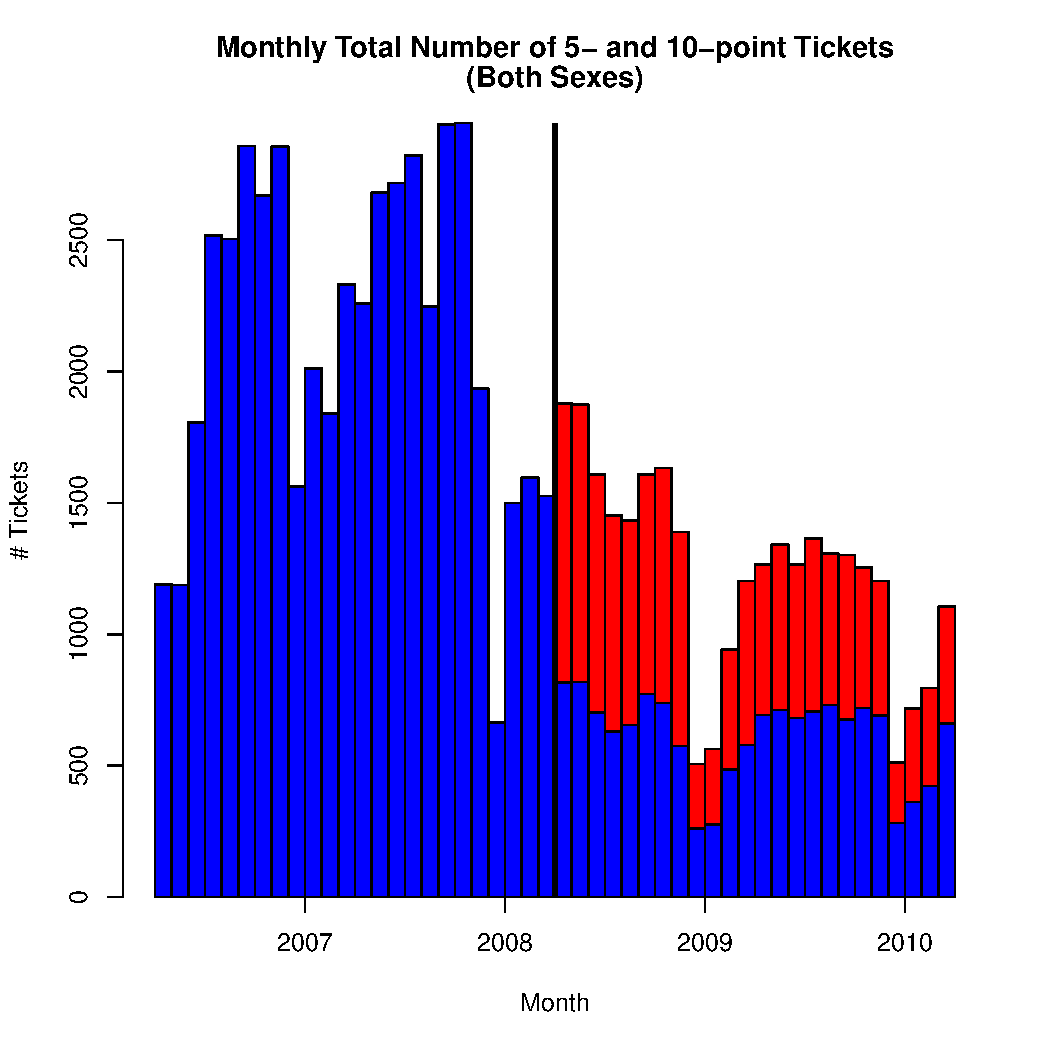
\includegraphics[width=0.8\textwidth]{../Figures/num_pts_5_10_all_orig.pdf}
\caption{Monthly frequency of 5- and 10-point violations }
Notes: Authors calculations. Monthly frequency of 5-point violations before the policy change and 5- or 10-point violations after the policy change. Blue areas correspond to 5 point-stops, while red areas are 10-point stops.
\label{fig:num_pts_5_10_all}
\end{figure}


\begin{figure}
\centering
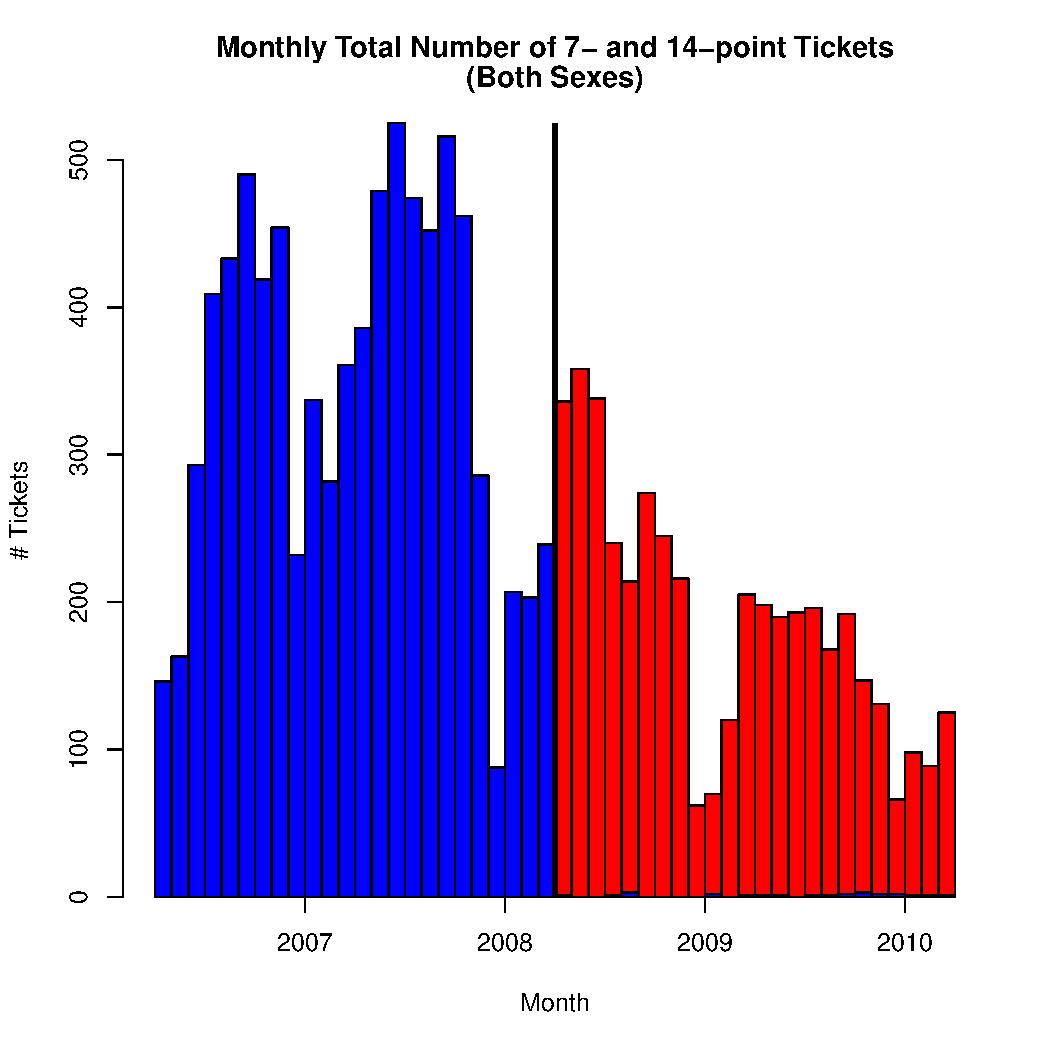
\includegraphics[width=0.8\textwidth]{../Figures/num_pts_7_14_all_orig.pdf}
\caption{Monthly frequency of 5- and 10-point violations }
Notes: Authors calculations. Monthly frequency of 7-point violations before the policy change and 7- or 14-point violations after the policy change. Blue areas correspond to 7-point stops, while red areas are 14-point stops.
\label{fig:num_pts_7_14_all}
\end{figure}




\begin{table}% [ht]
\centering
\begin{tabular}{r r r r r r r}
  \hline
		& \multicolumn{2}{c}{Both} 	&  \multicolumn{2}{c}{Males} &  \multicolumn{2}{c}{Females} \\
  \hline
points 	& pre 			& post			& pre 			& post			& pre 			& post		\\ 
  \hline

1		& 146,680		& 184,677		& 101,298		& 122,899		& 45,382		& 61,778    \\
2		& 782,836		& 855,302		& 533,167		& 572,194		& 249,669		& 283,108    \\
3		& 949,044		& 867,361		& 701,053		& 627,807		& 247,991		& 239,554    \\
4		& 17,783		& 17,748		& 15,567		& 15,278		& 2,216		& 2,470    \\
5		& 51,178		& 14,640		& 43,006		& 12,368		& 8,172		& 2,272    \\
6		& 517			& 15,296		& 496			& 12,000		& 21			& 3,296    \\
7		& 8,336		& 24			& 7,688		& 18			& 648			& 6    \\
9		& 9,969		& 8,222		& 7,382		& 5,791		& 2,587		& 2,431    \\
10		& 0				& 14,884		& 0				& 12,747		& 0				& 2,137    \\
12		& 128			& 0				& 127			& 0				& 1				& 0    \\
14		& 0				& 4,447		& 0				& 4,145		& 0				& 302    \\
15		& 18			& 0				& 17			& 0				& 1				& 0    \\
18		& 3				& 583			& 3				& 560			& 0				& 23    \\
24		& 0				& 102			& 0				& 98			& 0				& 4    \\
30		& 0				& 17			& 0				& 17			& 0				& 0    \\
36		& 0				& 4				& 0				& 4				& 0				& 0    \\

   \hline
Total 	& 1,966,492 	& 1,983,307 	& 1,409,804 	& 1,385,926 	& 556,688 		& 597,381 \\ 
   \hline
\end{tabular}
\caption{Frequency of tickets by point value} 
Notes: Author’s calculations. The pre and post columns refer to before and after the policy change.
\label{tab:penalties}
\end{table}




% Linear Probability Models: Original Specification 

\begin{table}% [ht] 
\centering 
\begin{tabular}{l r r l r r l} 

\hline 
 
 
 

\hline  

\end{tabular} 
\caption{Regressions} 
\label{tab:orig_regs} 
\end{table} 
 


% Linear Probability Models: Original LPM Specification by Point Value 

\begin{table}% [ht] 
\centering 
\begin{tabular}{l r r l r r l} 

\hline 
 
 & \multicolumn{3}{c}{Males} & \multicolumn{3}{c}{Females} \\ 

\hline 
 
 & Estimate & Std. Error & Sig. & Estimate & Std. Error & Sig. \\ 

\hline 
 
All point values                &  -5.92E-05        &  6.28E-07       &   **       &  -7.59E-06        &  4.95E-07       &   **       \\ 
1 points                        &  3.98E-06        &  1.77E-07       &   **       &  5.22E-06        &  1.50E-07       &   **       \\ 
2 points                        &  -4.11E-06        &  3.94E-07       &   **       &  3.81E-06        &  3.36E-07       &   **       \\ 
3 points                        &  -4.76E-05        &  4.36E-07       &   **       &  -1.41E-05        &  3.23E-07       &   **       \\ 
4 points                        &  -8.09E-07        &  6.62E-08       &   **       &  -1.01E-08        &  3.16E-08       &            \\ 
5 points                        &  -8.20E-06        &  9.95E-08       &   **       &  -2.11E-06        &  5.27E-08       &   **       \\ 
7 points                        &  -1.63E-06        &  4.17E-08       &   **       &  -1.92E-07        &  1.47E-08       &   **       \\ 
9 or more points                &  -6.75E-07        &  4.47E-08       &   **       &  -1.78E-07        &  3.29E-08       &   **       \\ 
Observations            & 5,335,033,221    &          &              &  4,340,212,273 \\ 


\hline 

\end{tabular} 
\caption{Regressions by ticket-point value (Original LPM)} 
All regressions contain age category and demerit point category controls. 
The symbol * denotes statistical significance at the 0.1\% level 
and ** the 0.001\% level. 
``Sig.'' is an abbreviation for statistical significance. 
Estimates and standard errors are in scientific notation. 
Heteroskedasticity-robust errors are employed. 
The baseline age category comprises drivers under the age of 16. 
The 5 point category of tickets includes 10 point tickets after the policy change,  
the 7 point category includes 14 point tickets after the policy change,  
and 9 or more point tickets include all possible doubled values for those tickets  
worth more than 9 points after the policy change. 
\label{tab:orig_regs_by_points} 
\end{table} 
 


% Linear Probability Models: Original High-Point Subsample 

\begin{table}% [ht] 
\centering 
\begin{tabular}{l r r l r r l} 

\hline 
 
 & Estimate & Std. Error & Sig. & Estimate & Std. Error & Sig. \\ 

\hline 
 
\textbf{Full sample} \\ 

Policy             &  -3.82E-05        &  4.11E-07       &   **       &  -1.12E-05        &  5.70E-06       &            \\ 
Age 16-19 * policy           & & &  &  -6.28E-05        &  6.71E-06       &   **       \\ 
Age 20-24 * policy           & & &  &  -6.81E-05        &  6.06E-06       &   **       \\ 
Age 25-34 * policy           & & &  &  -5.17E-05        &  5.81E-06       &   **       \\ 
Age 35-44 * policy           & & &  &  -2.70E-05        &  5.78E-06       &   **       \\ 
Age 45-54 * policy           & & &  &  -1.96E-05        &  5.76E-06       &    *       \\ 
Age 55-64 * policy           & & &  &  -1.23E-05        &  5.76E-06       &            \\ 
Age 65+ * policy           & & &  &  3.59E-06        &  5.75E-06       &            \\ 
Observations & 1,170,426,426 \\ 


\hline 

\textbf{Male} \\ 

Policy             &  -5.92E-05        &  6.28E-07       &   **       &  -1.04E-05        &  7.34E-06       &            \\ 
Age 16-19 * policy           & & &  &  -1.12E-04        &  9.19E-06       &   **       \\ 
Age 20-24 * policy           & & &  &  -1.20E-04        &  8.02E-06       &   **       \\ 
Age 25-34 * policy           & & &  &  -8.63E-05        &  7.54E-06       &   **       \\ 
Age 35-44 * policy           & & &  &  -5.04E-05        &  7.48E-06       &   **       \\ 
Age 45-54 * policy           & & &  &  -3.58E-05        &  7.45E-06       &   **       \\ 
Age 55-64 * policy           & & &  &  -2.53E-05        &  7.46E-06       &    *       \\ 
Age 65+ * policy           & & &  &  -2.91E-06        &  7.43E-06       &            \\ 
Observations & 921,131,812 \\ 


\hline 

\textbf{Female} \\ 

Policy             &  -7.59E-06        &  4.95E-07       &   **       &  -6.70E-06        &  6.35E-06       &            \\ 
Age 16-19 * policy           & & &  &  7.47E-06        &  7.41E-06       &            \\ 
Age 20-24 * policy           & & &  &  -8.99E-07        &  6.76E-06       &            \\ 
Age 25-34 * policy           & & &  &  -9.93E-06        &  6.48E-06       &            \\ 
Age 35-44 * policy           & & &  &  1.57E-07        &  6.46E-06       &            \\ 
Age 45-54 * policy           & & &  &  -2.16E-06        &  6.42E-06       &            \\ 
Age 55-64 * policy           & & &  &  9.92E-07        &  6.42E-06       &            \\ 
Age 65+ * policy           & & &  &  9.38E-06        &  6.42E-06       &            \\ 
Observations & 249,294,614 \\ 


\hline 

\end{tabular} 
\caption{Regressions for high-point drivers} 
All regressions contain age category and demerit point category controls. 
The symbol * denotes statistical significance at the 0.1\% level 
and ** the 0.001\% level. 
``Sig.'' is an abbreviation for statistical significance. 
Estimates and standard errors are in scientific notation. 
Heteroskedasticity-robust errors are employed. 
The baseline age category comprises drivers under the age of 16. 
\label{tab:orig_high_pt_regs} 
\end{table} 
 


% Linear Probability Models: Original Placebo Specification 

\begin{table}% [ht] 
\centering 
\begin{tabular}{l r r l r r l} 

\hline 
 
 & Estimate & Std. Error & Sig. & Estimate & Std. Error & Sig. \\ 

\hline 
 
\textbf{Full sample} \\ 

Policy             &  -3.87E-06        &  5.92E-07       &   **       &  -1.29E-05        &  8.06E-06       &            \\ 
Age 16-19 * policy           & & &  &  -1.91E-05        &  9.61E-06       &            \\ 
Age 20-24 * policy           & & &  &  9.64E-07        &  8.59E-06       &            \\ 
Age 25-34 * policy           & & &  &  6.16E-06        &  8.21E-06       &            \\ 
Age 35-44 * policy           & & &  &  4.05E-06        &  8.17E-06       &            \\ 
Age 45-54 * policy           & & &  &  1.15E-05        &  8.14E-06       &            \\ 
Age 55-64 * policy           & & &  &  1.51E-05        &  8.15E-06       &            \\ 
Age 65+ * policy           & & &  &  1.96E-05        &  8.14E-06       &            \\ 
Observations & 4,728,750,336 \\ 


\hline 

\textbf{Male} \\ 

Policy             &  -2.01E-06        &  9.06E-07       &            &  -1.80E-05        &  1.02E-05       &            \\ 
Age 16-19 * policy           & & &  &  -2.94E-05        &  1.31E-05       &            \\ 
Age 20-24 * policy           & & &  &  -1.01E-06        &  1.12E-05       &            \\ 
Age 25-34 * policy           & & &  &  1.34E-05        &  1.05E-05       &            \\ 
Age 35-44 * policy           & & &  &  1.24E-05        &  1.04E-05       &            \\ 
Age 45-54 * policy           & & &  &  1.98E-05        &  1.04E-05       &            \\ 
Age 55-64 * policy           & & &  &  2.33E-05        &  1.04E-05       &            \\ 
Age 65+ * policy           & & &  &  2.73E-05        &  1.03E-05       &            \\ 
Observations & 2,618,869,394 \\ 


\hline 

\textbf{Female} \\ 

Policy             &  -1.73E-06        &  7.07E-07       &            &  7.30E-06        &  9.25E-06       &            \\ 
Age 16-19 * policy           & & &  &  -1.16E-05        &  1.08E-05       &            \\ 
Age 20-24 * policy           & & &  &  -1.14E-06        &  9.82E-06       &            \\ 
Age 25-34 * policy           & & &  &  -1.06E-05        &  9.44E-06       &            \\ 
Age 35-44 * policy           & & &  &  -1.51E-05        &  9.40E-06       &            \\ 
Age 45-54 * policy           & & &  &  -8.68E-06        &  9.35E-06       &            \\ 
Age 55-64 * policy           & & &  &  -6.71E-06        &  9.36E-06       &            \\ 
Age 65+ * policy           & & &  &  -3.47E-06        &  9.34E-06       &            \\ 
Observations & 2,109,880,942  \\ 


\hline 

\end{tabular} 
\caption{Placebo regressions} 
All regressions contain age category and demerit point category controls. 
The symbol * denotes statistical significance at the 0.1\% level 
and ** the 0.001\% level. 
``Sig.'' is an abbreviation for statistical significance. 
Estimates and standard errors are in scientific notation. 
Heteroskedasticity-robust errors are employed. 
The baseline age category comprises drivers under the age of 16. 
\label{tab:orig_placebo_regs} 
\end{table} 
 



\pagebreak

\section*{Appendix B}
\vspace{3.0in}

\section*{Tables and Figures with Seasonality}
\label{sec:Appendix}

\vfill
\eject




